\chapter{Struttura del MagicMirror}\label{capitolo3}
Il MagicMirror (detto anche \emph{MM}) \`e un progetto ideato e sviluppato da Michael Teeuw, successivamente esteso nelle sue
funzionalit\`a da una moltitudine di utenti su GitHub.
La prima versione \`e stata scritta completamente in Python, mentre nella versione successiva \`e stato utilizzato Electron,
che ha comportato una variazione di linguaggio, a favore di Javascript. In questo modo \`e stato possibile implementare un'interfaccia esteticamente pi\`u gradevole
e API pi\`u intuitive.
L'idea dell'autore \`e nata rifacendosi allo specchio magico della rinomata fiaba
scritta dai fratelli Grimm: Biancaneve e i Sette Nani.\\
Il software viene mostrato attraverso un
comune monitor, trasmettendo immagini poste su uno sfondo completamente nero. Applicando sopra
una semplice pellicola a specchio (la quale da un lato permette di specchiarsi e dall'altro di vedere
attraverso) si crea un effetto particolare per cui una persona riesce a specchiarsi
e allo stesso tempo riesce a vedere le scritte o le immagini trasmesse dal monitor,
come mostrato in figura \ref{fig:MM}. In quest'ultima si pu\`o vedere il MM
che, oltre alla sua funzione base di specchio, mostra alcune informazioni come l'ora, la temperatura, il meteo e un messaggio.\\
In questo capitolo verr\`a spiegata la struttura generale del MM (sezione \ref{cap:MMalto}), le classi principali che vengono caricate
all'avvio (sezione \ref{cap:MMavvio}), la struttura del file di configurazione (sezione \ref{cap:MMconf}),
come viene implementata un'applicazione (sezione \ref{cap:app})
e il funzionamento del sistema di messaggistica (sezione \ref{cap:MMmess}).\\[2\baselineskip]
\begin{figure}[H]
    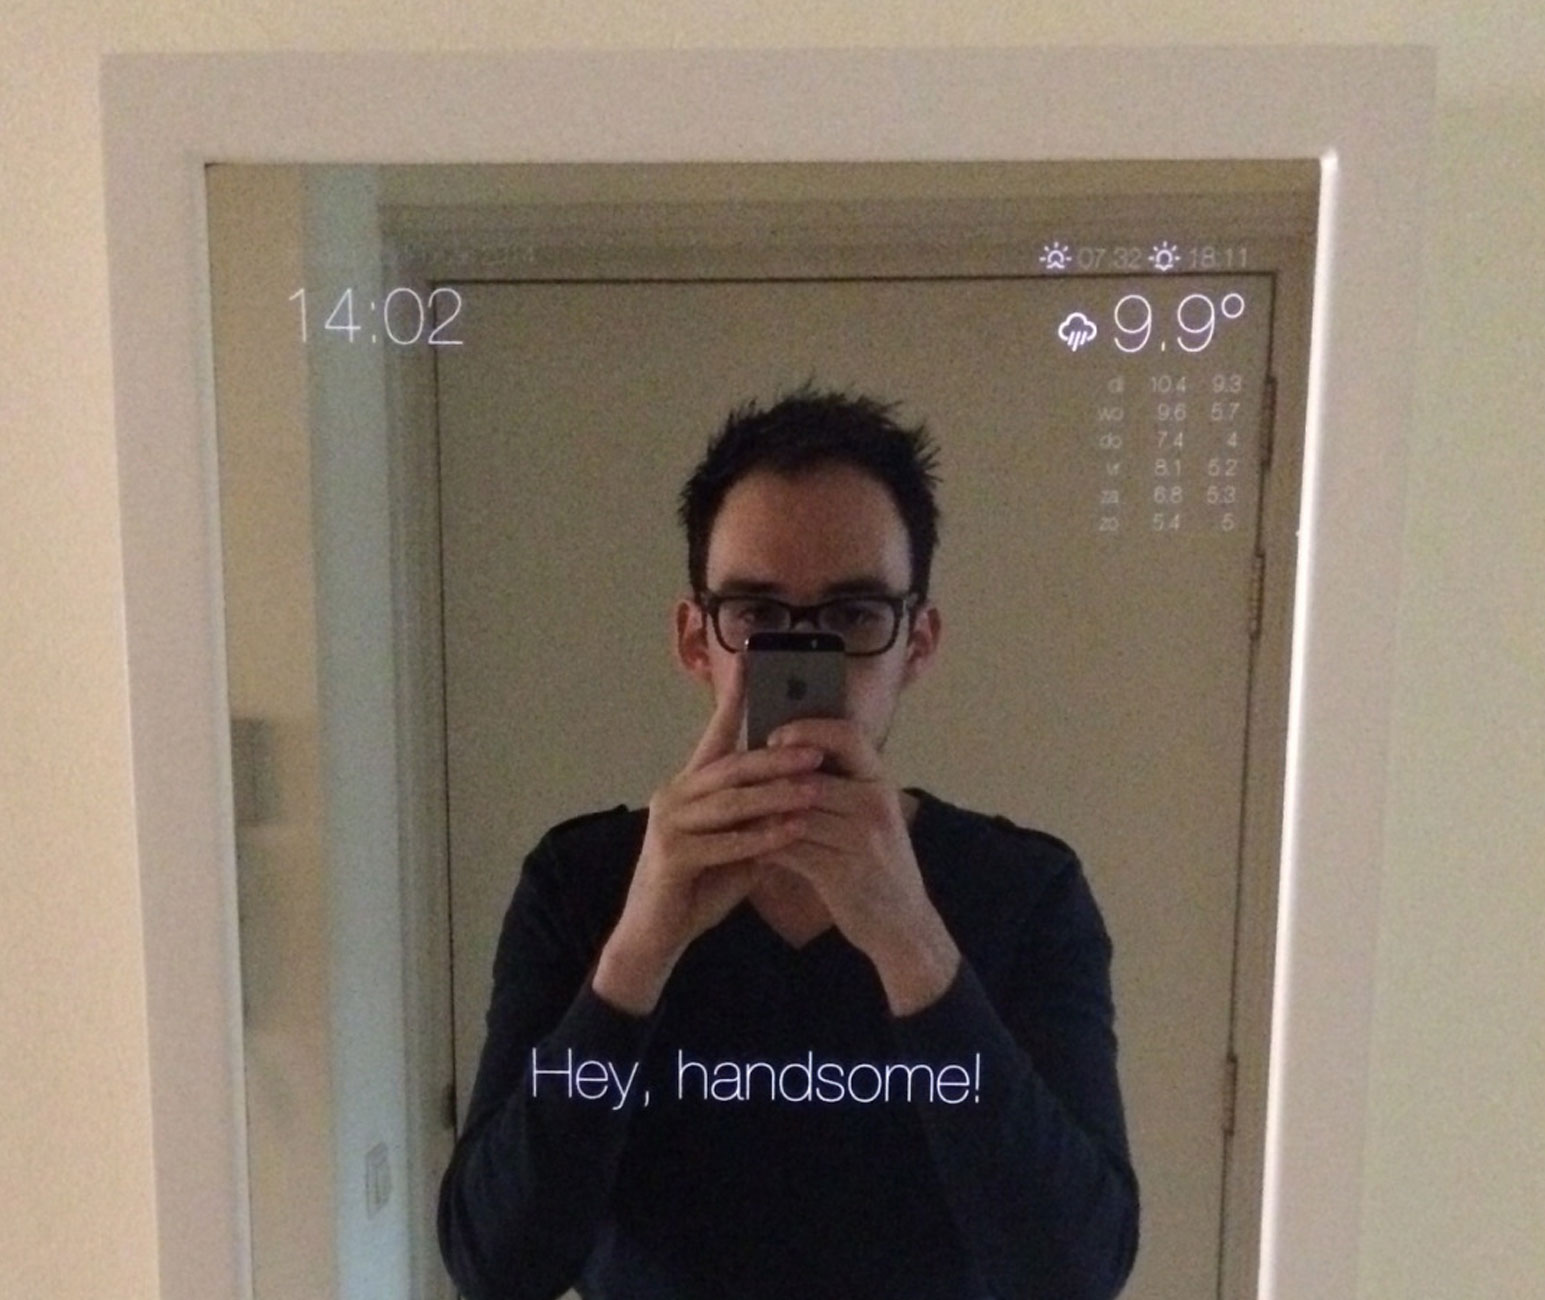
\includegraphics[width=1\textwidth, height=0.6\textheight]{magic_mirror}
    \caption{MagicMirror by Michael Teeuw}
    \label{fig:MM}
\end{figure}

\section{Il MM dall'alto livello}\label{cap:MMalto}
Il MM \`e una applicazione composta da diversi componenti software con cui \`e possibile
comunicare attraverso le API messe a disposizione da MM.
Si possono individuare alcuni elementi principali rappresentati in figura \ref{fig:struttMM}:
\begin{figure}[H]
    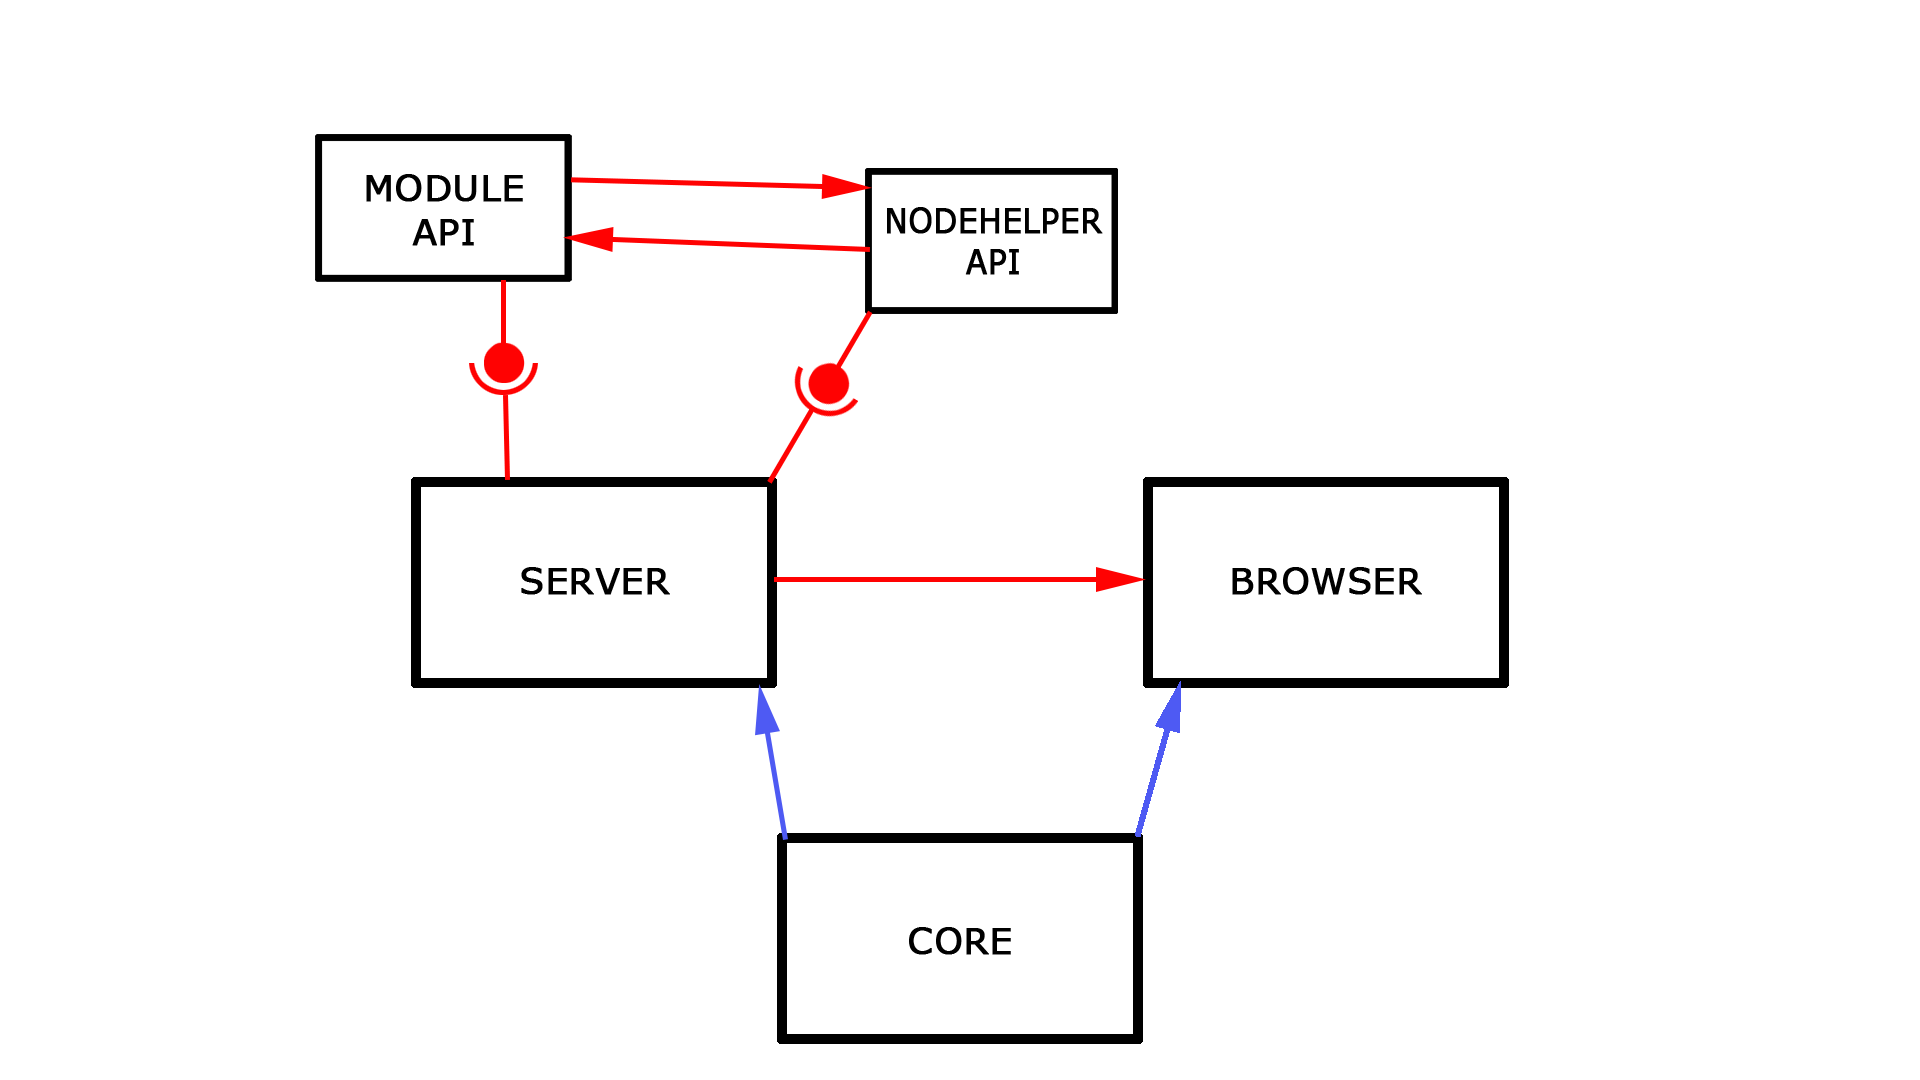
\includegraphics[width=1\textwidth, height=0.4\textheight]{strutturaMM}
    \caption{Struttura MagicMirror}
    \label{fig:struttMM}
\end{figure}
\begin{itemize}
\item Il core, il cuore del MM dove gira il codice principale.
\item Il server, che gira in locale, usato per restituire la pagina HTML, con i dati, al browser di Electron e comunicare con le API
\item I Moduli, entit\`a che espone le API per l'implementazione di applicazioni
\item I NodeHelper, entit\`a che espone le API per l'implementazione di funzioni di supporto al Modulo
\item Il Socket, entit\`a che fornisce un canale di comunicazione tra i Moduli
\item Il SocketClient, entit\`a che fornisce un canale di comunicazione tra un Modulo e il proprio NodeHelper.\\[2\baselineskip]
\end{itemize}

\section{Avvio ed Esecuzione}\label{cap:MMavvio}
Il MM viene avviato tramite linea di comando, la quale esegue
il codice di un file Javascript, il cui percorso \`e indicato nel documento \textit{package.json} di Electron, descritto nella sezione \ref{cap:Electron}.
Il file contiene il codice di Electron, che si occupa dell'avvio di MM, caricandone tutte le strutture, e della creazione di una nuova finestra browser,
il cui compito \`e di mostrare l'output dei moduli.
La pagina costruita e l'output dei moduli sono un insieme di Document Object Model (DOM), ovvero oggetti HTML che compongono una pagina web,
i quali vengono mostrati
solo dopo l'avvio di tutti i moduli attivi.\\
Le strutture principali caricate dal MM sono le seguenti:
\begin{itemize}
\item gli end-point delle API per le applicazioni, che sono le interfacce usate per leggere e caricare le applicazioni inserite nel MM.
\item gli end-point delle API per la gestione dei NodeHelper. Sono strutture opzionali usate per collegamenti
esterni al MM (per esempio, con API di un servizio cloud). Ogni applicazione ha il proprio NodeHelper con cui pu\`o comunicare tramite messaggi in modo
simile a come comunicano le applicazioni tra di loro.
\item un "Socket" e un "Socket-Client", entit\`a principali che definiscono le funzioni per lo scambio dei messaggi tra le applicazioni e i
rispettivi NodeHelper.
\item un Logger, implementato per tenere i log dell'applicazione e degli eventuali errori. Usato principalmente per il debugging.
\item un file di configurazione, nel quale sono specificati il nome e le coordinate per la posizione dei vari moduli
all'interno della pagina.\\[2\baselineskip]
\end{itemize}
Inoltre viene inizializzato un server, il cui compito \`e quello di trasmettere la pagina HTML generata, con gli output delle varie applicazioni,
al browser precedentemente avviato.

\subsection{Il file di Configurazione}\label{cap:MMconf}
Come discusso nella sezione \ref{cap:interfacciaproblemi}, il MM carica un file di configurazione, che \`e composto dai seguenti campi:
\begin{itemize}
\item la porta del server
\item una whitelist, ovvero un IP oppure un range di IP che possono collegarsi allo specchio
\item la lingua principale del sistema
\item il formato dell'ora (12h o 24h)
\item l'unit\`a di misura (ad esempio pixel), usata per gestire la distanza degli oggetti HTML
\item una lista di moduli (in formato JSON) da caricare durante l'avvio del MM con la relativa posizione nella pagina. Per ogni applicazione deve necessariamente comparire il
nome e la posizione; opzionalmente si possono inserire un campo  \textit{header} e un campo \textit{config} specifico per l'applicazione, come mostrato
nell'esempio in figura \ref{code:configapp}.
\begin{lstlisting}[label={code:configapp}, caption={Campi di configurazione di un modulo nel MM}, captionpos=b]
{
	"module": 'nome dell'applicazione',
	"position": 'la posizione dell'applicazione all'intenro dello specchio',
	"header": 'una stringa che viene stampata sopra all'applicazione',
	"config": { opzioni varie in formato JSON }
}
\end{lstlisting}
\end{itemize}
La lingua, il formato dell'ora e l'unit\`a di misura usata sono parametri messi a disposizione dal sistema per la creazione di un'applicazione
(ad esempio, il display di un orologio).

\section{Implementazione di un'applicazione}\label{cap:app}
La modifica del file di configurazione del MM appena descritta serve per "notificare" la presenza delle applicazioni a quest'ultimo,
ma perch\`e possano funzionare \`e necessario che rispettino alcune specifiche regole.
Per inserire il codice dell'applicazione all'interno dello specchio \`e necessario creare una cartella con un nome identificativo dell'applicazione
nella directory \textit{Modules}.
Dentro la cartella appena creata devono essere inseriti:
\begin{itemize}
\item 1 file Javascript (JS), ovvero il documento principale con lo stesso nome della cartella appena creata. Contiene il codice dell'applicazione, il quale
conterr\`a a sua volta il codice per la creazione dei DOM
\item 1 file Cascading Style Sheets (CSS), per modificare l'estetica del DOM della relativa applicazione (opzionale)
\item 1 file node\_helper.js, che \`e il NodeHelper associato alla specifica applicazione (opzionale)
\item Altri file necessari all'applicazione (immagini, JSON, etc)\\[1\baselineskip]
\end{itemize}



\iffalse
Le funzioni offerte dalle API sono:
\begin{itemize}
\item defaults: {}, una lista di variabili che possono essere richiamate all'interno di una qualsiasi funzione tramite il comando \textit{this.config.variabile}.
I valori di queste possono essere sovrascritti modificando il campo \textit{config} del relativo modulo nel file di configurazione del MM.
\item start: function(){}, funzione che viene eseguita quando tutte le applicazioni dello specchio sono state caricate (ovvero quando sono stati creati tutti i relativi DOM)
\item getDom: function(){}, funzione che deve ritornare un DOM (un oggetto HTML contenente i dati da mostrare a schermo), creato tramite funzioni Javascript
\item getStyles: function() { return []}, funzione che ritorna un array di file (in formato CSS) usati per l'estetica del DOM. Possono essere nella cartella dell'applicazione
oppure ottenuti tramite link
\item getTranslations: function() {	return {en: "translations/en.json", de: "translations/de.json"}}, funzione per tradurre l'applicazione in pi\`u lingue;
se disponibile, viene caricata la traduzione in base alla lingua configurata nel software
\item getHeader: function() {	return this.data.header;}, funzione che stampa il campo \textit{header} della configurazione, con la possibilit\`a concaternarla
ad una stringa o ad un parametro
\item notificationReceived: function(notification, payload, sender) {}, funzione che serve per ricevere messaggi da altre applicazioni. Viene richiamata alla ricezione
\item socketNotificationReceived: function(notification, payload){}, funzione che serve per ricevere messaggi dal NodeHelper della relativa applicazione\\[1\baselineskip]
\end{itemize}
Inoltre possono essere aggiunte delle funzioni necessarie all'applicazione implementandole con la stessa sintassi di quelle di default.
\\[1\baselineskip]
Il NodeHelper, invece, viene caricato come libreria ed esportato insieme all'applicazione quando viene caricata dallo specchio. Per inizializzarlo sono
necessari i comandi:
\begin{lstlisting}[language=JavaScript]
{
  var NodeHelper = require("node_helper");
  module.exports = NodeHelper.create({/* lista JSON di oggetti contenenti funzioni*/});
}
\end{lstlisting}
A differenza del file Javascript principale, l'unica funzione messa a disposizione dall' API \`e:
\begin{lstlisting}[language=JavaScript]
{
  start: function() {}
}
\end{lstlisting}
mentre \`e possibile implementare le proprie funzioni con la stessa sintassi.
\fi


\section{Messaggistica del MM}\label{cap:MMmess}
Nella sezione \ref{cap:MMalto} \`e stato gi\`a accennato che il MM implementa un meccanismo di messaggistica sfruttando un sistema di socket integrato,
utile per l'organizzazione e la moderazione delle applicazioni tramite l'utilizzo di funzioni messe a disposizione dall'API.
Sono presenti due classi socket:
\begin{itemize}
\item Socket, classe che fornisce le funzioni per ricevere e mandare messaggi tra i moduli del MM. Con questo socket la spedizione
del messaggio \`e in broadcast usando il metodo \textit{sendNotification(notification, payload)}. Il primo parametro \`e una stringa che identifica
il messaggio, il secondo parametro \`e opzionale e pu\`o essere usato per inserire il corpo del messaggio.
La ricezione del messaggio viene gestita con il metodo \textit{notificationReceived(notification, payload, sender)}, i primi due parametri sono
uguali a quelli della funzione per spedire, il terzo parametro contiene il nome del
modulo che ha mandato il messaggio
\item SocketClient, classe che fornisce le funzioni per ricevere e mandare messaggi tra il modulo e il suo NodeHelper. Per spedire
i messaggi viene usata la funzione \textit{sendSocketNotification(notification, payload)}, mentre la ricezione viene gestita con la funzione
 \textit{socketNotificationReceived(notification, payload)}. I campi di queste due funzioni sono gli stessi descritti nel punto precedente.\\[1\baselineskip]
\end{itemize}
